\documentclass[tikz, border=8pt]{standalone}
\usepackage{xcolor}
\usetikzlibrary{arrows.meta, positioning, shapes.geometric, calc}
% ============================================================
% Shared style definitions for the DarwinsRNAHunt methods figures.
% \input this file from each diagram's preamble (after \usepackage{xcolor}
% and \usetikzlibrary{...}) so colours/styles stay consistent everywhere.
%
% Visual grammar used throughout:
%   - white box, single border   = external / raw resource
%   - white box, double border   = curated data artifact (output of a section)
%   - coloured box, single border = an internal processing step
%   - coloured/white, dashed border = Snakemake checkpoint (dynamic re-evaluation)
%   - white box, short-dashed border = static external file (not produced by the pipeline)
% ============================================================

% ---------- category colours (ColorBrewer Set3-style) ----------
\definecolor{catDefine}{HTML}{FFFFFF}
\definecolor{catSelect}{HTML}{FFFFFF}
\definecolor{catAcquire}{HTML}{FFFFFF}
\definecolor{catLocalize}{HTML}{FFFFFF}
\definecolor{catExtract}{HTML}{FFFFFF}
\definecolor{catCombine}{HTML}{FFFFFF}
\definecolor{catCluster}{HTML}{FFFFFF}
\definecolor{catModel}{HTML}{FFFFFF}
\definecolor{catValidate}{HTML}{FFFFFF}
\definecolor{catReport}{HTML}{FFFFFF}

% ---------- Kea Palette (defined for optional future restyling; unused for now) ----------
\definecolor{keaGreen}{HTML}{6C803A}
\definecolor{darkBrown}{HTML}{7B5C34}
\definecolor{lightBrown}{HTML}{AB7C47}
\definecolor{keaYellow}{HTML}{CCAE42}
\definecolor{keaOrange}{HTML}{D73202}
\definecolor{charcoal}{HTML}{272318}
\definecolor{lightGrey}{HTML}{D3CDBF}

\tikzset{
    font=\fontsize{7}{8}\selectfont,
    >={Latex[length=2mm,width=1.4mm]},
    every path/.style={thick},
    % internal processing step
    stage/.style={rectangle, rounded corners=2pt, draw=black, thin,
        minimum height=1.05cm, text width=3.6cm, align=center, inner sep=3pt},
    % external / raw resource (input)
    res/.style={rectangle, rounded corners=2pt, draw=black, thin, fill=white,
        minimum height=1cm, text width=4.2cm, align=center, inner sep=3pt},
    % static external file, not produced by this pipeline
    ext/.style={rectangle, rounded corners=2pt, draw=black!55, dash pattern=on 2.2pt off 1.6pt,
        thin, minimum height=0.85cm, text width=3.1cm, align=center, fill=white,
        font=\fontsize{6.3}{7.3}\selectfont, inner sep=2.5pt},
    % Snakemake checkpoint modifier (combine with stage/res)
    ckpt/.style={dashed, line width=0.9pt},
    % deliverable / output-artifact modifier: crosses a section boundary
    deliver/.style={double, double distance=1.2pt, line width=0.85pt},
    lbl/.style={font=\fontsize{8.5}{9.5}\bfseries\selectfont},
    sublbl/.style={font=\fontsize{7}{8}\itshape\selectfont},
    node distance=0.55cm and 2.6cm
}


\begin{document}
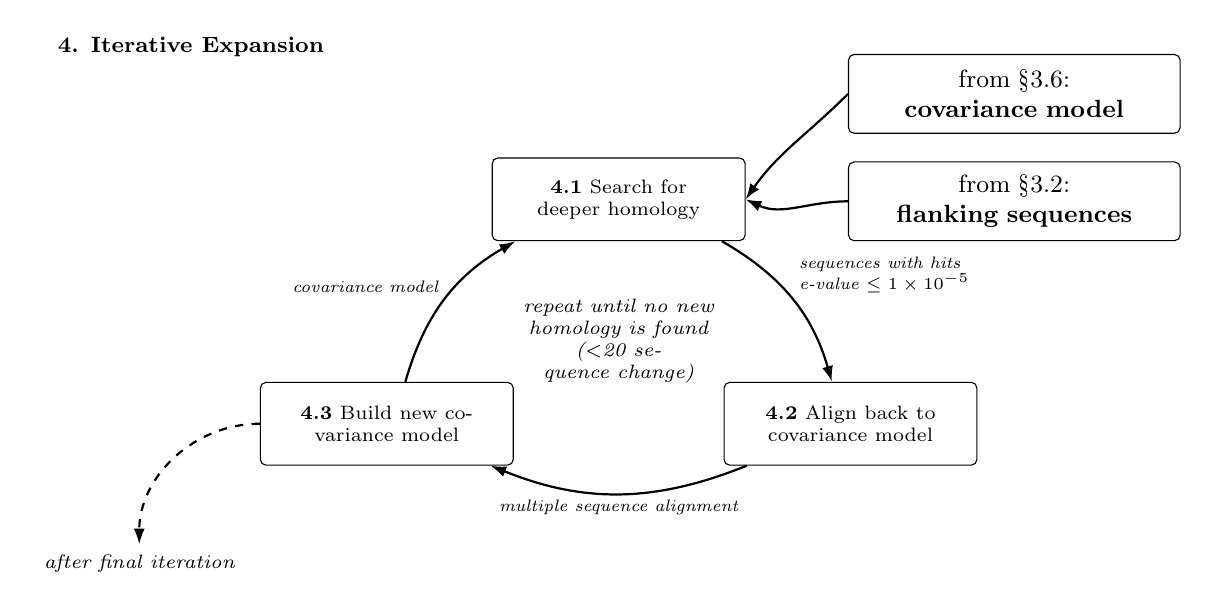
\begin{tikzpicture}[
    loopstage/.style={stage, fill=catModel!60, text width=3.0cm},
    edgelab/.style={font=\fontsize{6.5}{7.5}\selectfont\itshape, inner sep=2pt},
]

% ---------------- the loop ----------------
\node[loopstage] (s41) at ({3.4*cos(90)},{1.9*sin(90)})   {\textbf{4.1} Search for deeper homology};
\node[loopstage] (s42) at ({3.4*cos(-30)},{1.9*sin(-30)}) {\textbf{4.2} Align back to covariance model};
\node[loopstage] (s43) at ({3.4*cos(210)},{1.9*sin(210)}) {\textbf{4.3} Build new covariance model};

\draw[->, thick] (s41) to[bend left=22]
    node[edgelab, midway, above right, align=left] {sequences with hits\\e-value $\leq 1\times10^{-5}$} (s42);
\draw[->, thick] (s42) to[bend left=22]
    node[edgelab, midway, below, align=center] {multiple sequence alignment} (s43);
\draw[->, thick] (s43) to[bend left=22]
    node[edgelab, midway, above left, align=right] {covariance model} (s41);

\node[sublbl, text width=2.7cm, align=center] at (0,0.1)
    {repeat until no new homology is found\\($<$20 sequence change)};

% ---------------- header ----------------
\node[lbl, above left=1.15cm and 2cm of s41] (ie) {4. Iterative Expansion};

% ---------------- entry ----------------
\node[res, text width=4.0cm, font=\small, above right=0.3cm and 1.3cm of s41] (ctx)
    {from \S3.6:\\\textbf{covariance model}};
\node[res, text width=4.0cm, font=\small, below=0.35cm of ctx] (ctx2)
    {from \S3.2:\\\textbf{flanking sequences}};
\draw[->] (ctx.west) to[out=225, in=55] (s41.east);
\draw[->] (ctx2.west) to[out=180, in=-25] (s41.east);

% ---------------- exit ----------------
\node[sublbl, text width=2.6cm, align=center, below left=1cm and 0.1cm of s43] (exit) {after final iteration};
\draw[->, dashed] (s43.west) to[out=180, in=90] (exit.north);

\end{tikzpicture}
\end{document}